% hitex-deck-style: 2
\documentclass[aspectratio=169,11pt]{beamer}
\graphicspath{{../}}
\usetheme{default}
\usepackage{graphicx}
\usepackage{amsmath}
\usepackage{amssymb}
\usepackage{booktabs}
\usepackage{tikz}
\definecolor{hxStructure}{HTML}{1F497D}
\definecolor{hxAccent}{HTML}{C0392B}
\definecolor{hxMuted}{HTML}{696969}
\definecolor{hxText}{HTML}{000000}
\definecolor{hxBackground}{HTML}{FFFFFF}
\definecolor{hxTitleBg}{HTML}{F3F6FA}
\definecolor{hxTitleFg}{HTML}{1F497D}
\definecolor{hxRule}{HTML}{C7D2DE}
\definecolor{hxTint}{HTML}{A1B3C8}
\setbeamercolor{normal text}{fg=hxText,bg=hxBackground}
\setbeamercolor{background canvas}{bg=hxBackground}
\setbeamercolor{structure}{fg=hxStructure}
\setbeamercolor{title}{fg=hxStructure}
\setbeamercolor{frametitle}{fg=hxStructure}
\setbeamercolor{subtitle}{fg=hxMuted}
\setbeamercolor{author}{fg=hxText}
\setbeamercolor{alerted text}{fg=hxAccent}
\setbeamercolor{page number in head/foot}{fg=hxMuted}
\setbeamercolor{itemize item}{fg=hxStructure}
\setbeamercolor{itemize subitem}{fg=hxMuted}
\setbeamerfont{title}{series=\bfseries}
\setbeamerfont{frametitle}{series=\bfseries}
\setbeamertemplate{navigation symbols}{}
\setbeamertemplate{itemize item}{\raisebox{0.12em}{\rule{0.4em}{0.4em}}}
\setbeamertemplate{itemize subitem}{\textendash}
\makeatletter
\newcommand{\hxframes}{27}
% n / N: the total from the last run, or this deck's own count before there is one
\newcommand{\hxtotal}{\ifnum\inserttotalframenumber<\insertframenumber\relax\hxframes\else\inserttotalframenumber\fi}
\setbeamertemplate{frametitle}{%
  \vskip0.45cm%
  \begin{beamercolorbox}[wd=\paperwidth,leftskip=1cm,rightskip=1cm plus 1fil,sep=0pt]{frametitle}%
    \usebeamerfont{frametitle}\insertframetitle\par
    \ifx\insertframesubtitle\@empty\else{\small\color{hxMuted}\insertframesubtitle\par}\fi
    \nointerlineskip\vskip5pt{\color{hxAccent}\rule{1.2cm}{2.5pt}}\par
  \end{beamercolorbox}}
\setbeamertemplate{footline}{%
  \hbox to \paperwidth{\hskip1cm{\color{hxRule}\rule{\dimexpr\paperwidth-2cm\relax}{0.4pt}}\hss}%
  \vskip3pt%
  \hbox to \paperwidth{\hskip1cm\usebeamerfont{page number in head/foot}\usebeamercolor[fg]{page number in head/foot}%
    \insertshorttitle\hfill\insertframenumber\,/\,\hxtotal\hskip1cm}%
  \vskip6pt}
% Title, section and closing slides: a plain frame whose page background is drawn once by \hx@bg.
\let\hx@bg\@empty
\setbeamertemplate{background}{\ifx\hx@bg\@empty\else\hx@bg\global\let\hx@bg\@empty\fi}
% The title and closing slides: the title art (title-art.jpg, next to this file) full-bleed, its left
% side already the title background, and the text set on it on the left.
\newcommand*{\hxpresenter}{}
\newcommand*{\hxcoauthors}{}
\newcommand{\hx@art}[1]{%
  \IfFileExists{title-art.jpg}%
    {\node[anchor=south west,inner sep=0] at (0,0) {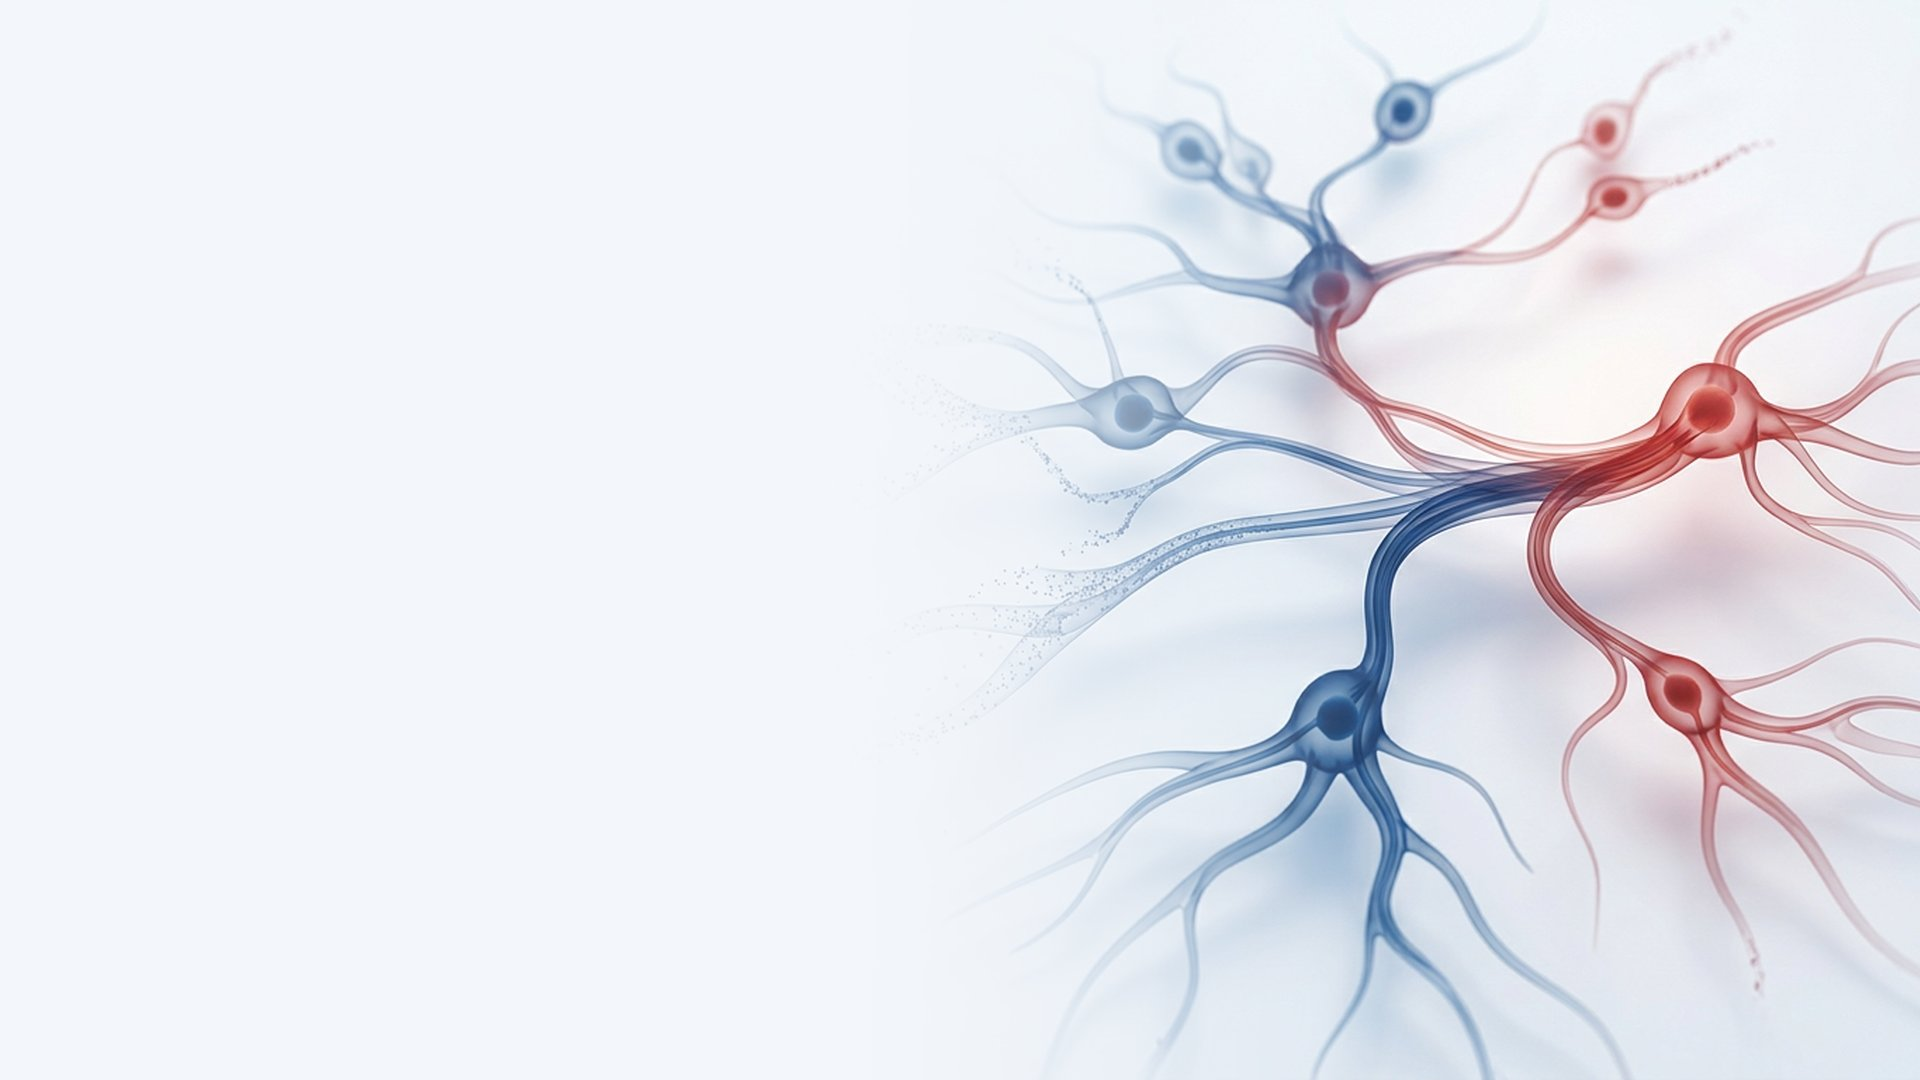
\includegraphics[width=\paperwidth,height=\paperheight]{title-art.jpg}};}%
    {\fill[hxTitleBg] (0,0) rectangle (\paperwidth,\paperheight);}%
  \ifnum#1=1 \fill[hxTitleBg,opacity=0.3] (0,0) rectangle (\paperwidth,\paperheight);\fi}
% Fitting: the title block hangs from 1.2 cm below the top, the author block stands on 0.9 cm above the
% bottom, with at least 0.6 cm (and the accent rule) between them. Measured in saveboxes in one pass;
% when they do not fit: affiliations \tiny, then co-authors \footnotesize, then the title block scaled
% (down to 60 %), then the whole stack scaled.
\newsavebox\hx@titlebox
\newsavebox\hx@authbox
\newdimen\hx@colw
\newdimen\hx@avail
\newdimen\hx@th
\newdimen\hx@ah
\newcommand{\hx@nohyph}{\hyphenpenalty=10000\exhyphenpenalty=10000\raggedright}
\newcommand{\hx@buildtitle}[2]{% #1 title, #2 subtitle (may be empty)
  \sbox\hx@titlebox{\parbox[t]{\hx@colw}{\hx@nohyph
    {\color{hxTitleFg}\huge\bfseries #1\par}%
    \ifx#2\@empty\else\vskip6pt{\color{hxText}\large\bfseries #2\par}\fi}}%
  \hx@th=\ht\hx@titlebox \advance\hx@th by \dp\hx@titlebox}
\newcommand{\hx@buildauthors}[2]{% #1 co-author size, #2 affiliation size
  \sbox\hx@authbox{\parbox[b]{\hx@colw}{\hx@nohyph\color{hxText}%
    {\bfseries\hxpresenter\par}%
    \ifx\hxcoauthors\@empty\else\vskip2pt{#1\hxcoauthors\par}\fi
    \ifx\insertinstitute\@empty\else\vskip4pt{#2\color{hxMuted}\insertinstitute\par}\fi}}%
  \hx@ah=\ht\hx@authbox \advance\hx@ah by \dp\hx@authbox}
\newcommand{\hx@fits}{\dimexpr\hx@th+\hx@ah\relax<\hx@avail}
\newcommand{\hxtitleslide}{\gdef\hx@bg{%
  \hx@colw=0.6\paperwidth
  \hx@avail=\paperheight \advance\hx@avail by -2.7cm \advance\hx@avail by -8.5pt
  \hx@buildtitle{\inserttitle}{\insertsubtitle}%
  \hx@buildauthors{\small}{\scriptsize}%
  \ifdim\hx@fits\else\hx@buildauthors{\small}{\tiny}\fi
  \ifdim\hx@fits\else\hx@buildauthors{\footnotesize}{\tiny}\fi
  \gdef\hx@ts{1}\gdef\hx@as{1}%
  \ifdim\hx@fits\else
    \pgfmathsetmacro\hx@ts{max(0.6,(\hx@avail-\hx@ah)/max(\hx@th,1pt))}%
    \pgfmathparse{(\hx@ts*\hx@th+\hx@ah) > \hx@avail ? 1 : 0}%
    \ifnum\pgfmathresult>0
      \pgfmathsetmacro\hx@as{\hx@avail/(0.6*\hx@th+\hx@ah)}%
      \pgfmathsetmacro\hx@ts{0.6*\hx@as}%
    \fi
  \fi
  \begin{tikzpicture}
  \useasboundingbox (0,0) rectangle (\paperwidth,\paperheight);
  \hx@art{0}
  \node[anchor=north west,inner sep=0] at (1cm,\paperheight-1.2cm) {\scalebox{\hx@ts}{\usebox\hx@titlebox}};
  \node[anchor=south west,inner sep=0] (hxauthors) at (1cm,0.9cm) {\scalebox{\hx@as}{\usebox\hx@authbox}};
  \fill[hxAccent] ([yshift=7pt]hxauthors.north west) rectangle +(1.2cm,1.5pt);
  \end{tikzpicture}}}
\newcommand{\hxclosingslide}[2]{\gdef\hx@bg{%
  \hx@colw=0.6\paperwidth
  \hx@avail=\paperheight \advance\hx@avail by -2.1cm
  \sbox\hx@titlebox{\parbox[t]{\hx@colw}{\hx@nohyph
    {\color{hxTitleFg}\huge\bfseries #1\par}\vskip9pt{\color{hxAccent}\rule{1.2cm}{1.5pt}}\par\vskip6pt
    {\color{hxText}\large #2\par}}}%
  \hx@th=\ht\hx@titlebox \advance\hx@th by \dp\hx@titlebox
  \gdef\hx@ts{1}%
  \ifdim\hx@th>\hx@avail \pgfmathsetmacro\hx@ts{\hx@avail/\hx@th}\fi
  \begin{tikzpicture}
  \useasboundingbox (0,0) rectangle (\paperwidth,\paperheight);
  \hx@art{1}
  % the block's top at 24 % of the height, raised (to 1.2 cm) and then scaled when it is taller
  \pgfmathsetmacro\hx@top{min(0.24*\paperheight, max(1.2cm, \paperheight-0.9cm-\hx@ts*\hx@th))}%
  \node[anchor=north west,inner sep=0] at (1cm,\paperheight-\hx@top pt) {\scalebox{\hx@ts}{\usebox\hx@titlebox}};
  \end{tikzpicture}}}
\newcommand{\hxsectionslide}[2]{\gdef\hx@bg{%
  \begin{tikzpicture}
  \useasboundingbox (0,0) rectangle (\paperwidth,\paperheight);
  \fill[hxStructure] (0,0) rectangle (0.3cm,\paperheight);
  \node[anchor=south west,inner sep=0,text=hxTint] at (1.6cm,0.5\paperheight+0.1cm)
    {\scalebox{2.2}{\Huge\bfseries #1}};
  \node[anchor=north west,inner sep=0,text width=\paperwidth-3.2cm,align=left,text=hxStructure]
    at (1.6cm,0.5\paperheight-0.25cm) {\hyphenpenalty=10000\exhyphenpenalty=10000\LARGE\bfseries #2\par};
  \end{tikzpicture}}}
\makeatother

\title[Benchmarking Single-Cell Marker-State Forecasting]{Benchmarking Single-Cell Marker-State Forecasting}
\subtitle{How cell coupling determines what benchmarks can detect}
\author{Victor Ikenna Kanu, Ihunanya Udodiri Ajakwe, Josiah Ayoola Isong, Simeon Okechukwu Ajakwe, Dong-Seong Kim}
\institute{Kumoh National Institute of Technology, Gumi, South Korea\\Kyungdong University, South Korea}
\renewcommand*{\hxpresenter}{Victor Ikenna Kanu}
\renewcommand*{\hxcoauthors}{Ihunanya Udodiri Ajakwe, Josiah Ayoola Isong, Simeon Okechukwu Ajakwe, Dong-Seong Kim}
\date{}

\begin{document}

\begin{frame}[plain]
\hxtitleslide
\end{frame}

\begin{frame}{Outline}
\large
\textcolor{hxAccent}{\textbf{01}}\hspace{0.8em}\textcolor{hxStructure}{Motivation}\par\medskip
\textcolor{hxAccent}{\textbf{02}}\hspace{0.8em}\textcolor{hxStructure}{Problem}\par\medskip
\textcolor{hxAccent}{\textbf{03}}\hspace{0.8em}\textcolor{hxStructure}{Approach}\par\medskip
\textcolor{hxAccent}{\textbf{04}}\hspace{0.8em}\textcolor{hxStructure}{Key results}\par\medskip
\textcolor{hxAccent}{\textbf{05}}\hspace{0.8em}\textcolor{hxStructure}{Takeaways}\par\medskip
\end{frame}

\section{Motivation}
\begin{frame}[plain]
\hxsectionslide{01}{Motivation}
\end{frame}

\begin{frame}{Forecasting differentiation states}
\begin{itemize}
\setlength{\itemsep}{0.6em}
\item{} Single-cell snapshots reveal stage-dependent differentiation programs
\item{} Forecasting asks whether early states predict later states
\item{} Model capacity should help only when temporal information exists
\end{itemize}
\end{frame}

\begin{frame}{The hidden benchmark assumption}
\begin{itemize}
\setlength{\itemsep}{0.6em}
\item{} Destructive measurement prevents observing the same cell across stages
\item{} Pseudo-trajectories concatenate cells from separate snapshots
\item{} Their coupling determines whether temporal dependence exists
\end{itemize}
\end{frame}

\begin{frame}{The central research question}
\begin{itemize}
\setlength{\itemsep}{0.6em}
\item{} Can a benchmark distinguish model skill from coupling artifacts?
\item{} Does a Transformer outperform simpler predictors?
\item{} Can a rigorous protocol recover both nulls and genuine dependence?
\end{itemize}
\end{frame}

\section{Problem}
\begin{frame}[plain]
\hxsectionslide{02}{Problem}
\end{frame}

\begin{frame}{Two differentiation systems}
\begin{columns}[c]
\begin{column}{0.56\textwidth}
\centering
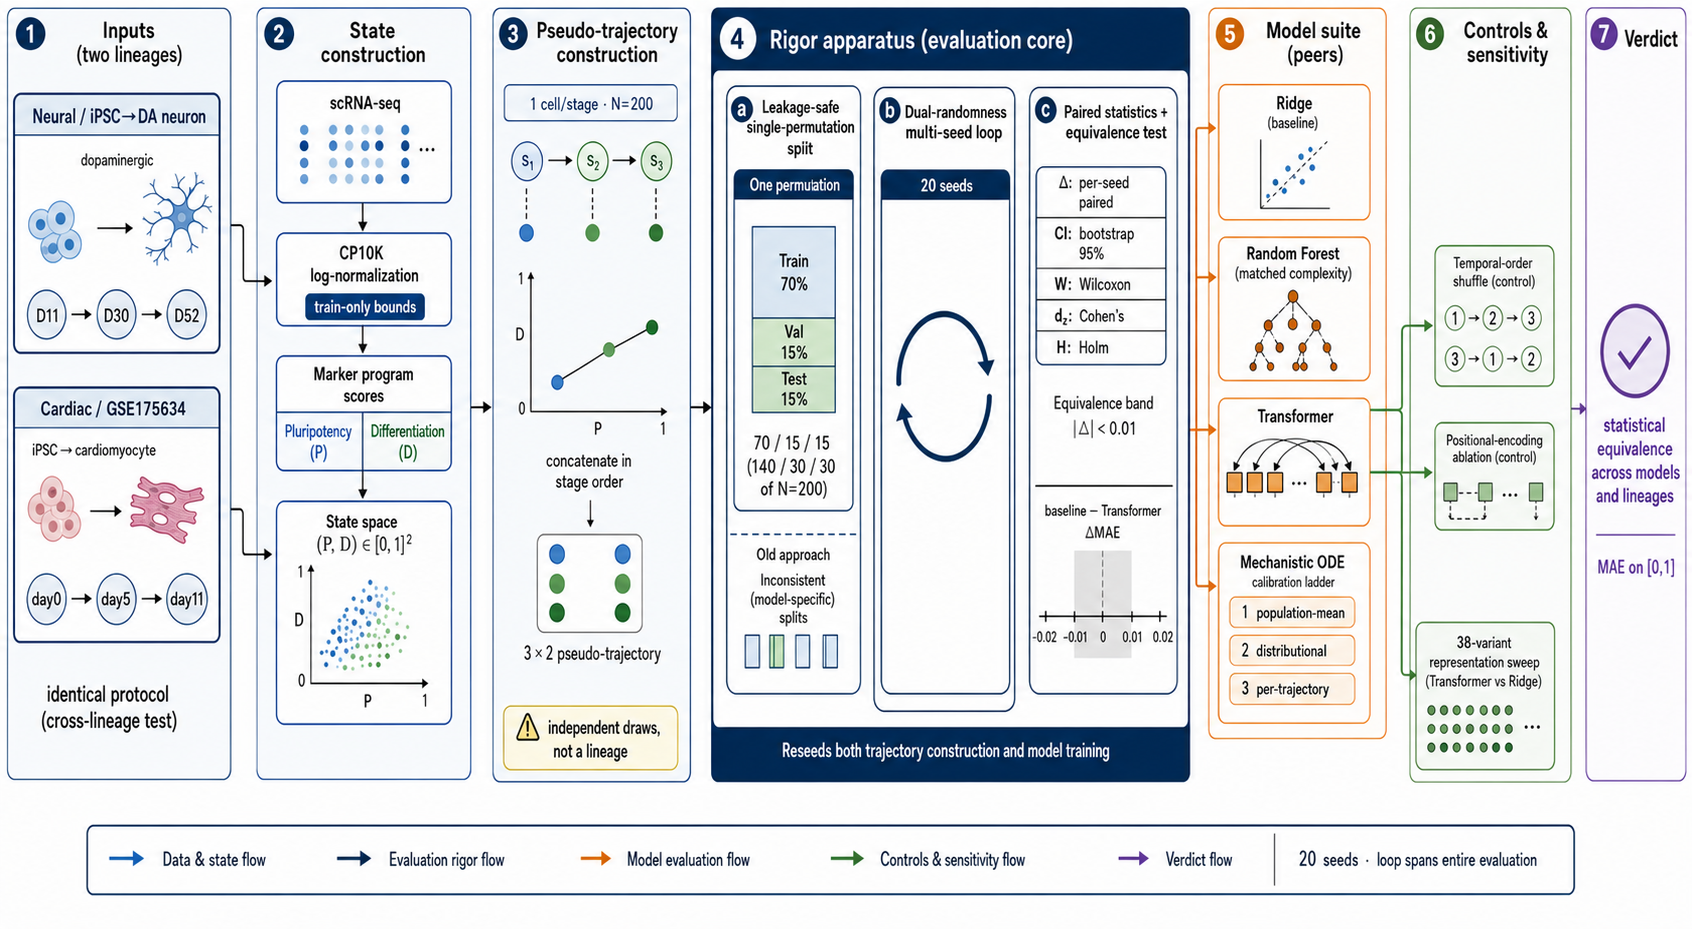
\includegraphics[width=\linewidth,height=0.78\textheight,keepaspectratio]{figures/method_design.png}
\end{column}
\begin{column}{0.41\textwidth}
\small
\begin{itemize}
\setlength{\itemsep}{0.6em}
\item{} Neural: iPSC to dopaminergic neuron, days 11, 30, and 52
\item{} Cardiac: iPSC to cardiomyocyte, days 0, 5, and 11
\item{} Each cell becomes a two-dimensional marker-state representation
\end{itemize}
\end{column}
\end{columns}
\end{frame}

\begin{frame}{Independent pairing creates a null}
\begin{itemize}
\setlength{\itemsep}{0.6em}
\item{} Each stage contributes an independent sampled cell
\item{} The late state is independent of earlier states
\item{} The absolute-error optimum is the constant training median
\end{itemize}
\end{frame}

\begin{frame}{What must evaluation prevent?}
\begin{itemize}
\setlength{\itemsep}{0.6em}
\item{} Train-test leakage can manufacture apparent model advantages
\item{} Single seeds cannot separate effects from sampling variation
\item{} Nonsignificance alone does not establish equivalence
\end{itemize}
\end{frame}

\section{Approach}
\begin{frame}[plain]
\hxsectionslide{03}{Approach}
\end{frame}

\begin{frame}{A leakage-safe benchmark}
\begin{columns}[c]
\begin{column}{0.56\textwidth}
\centering
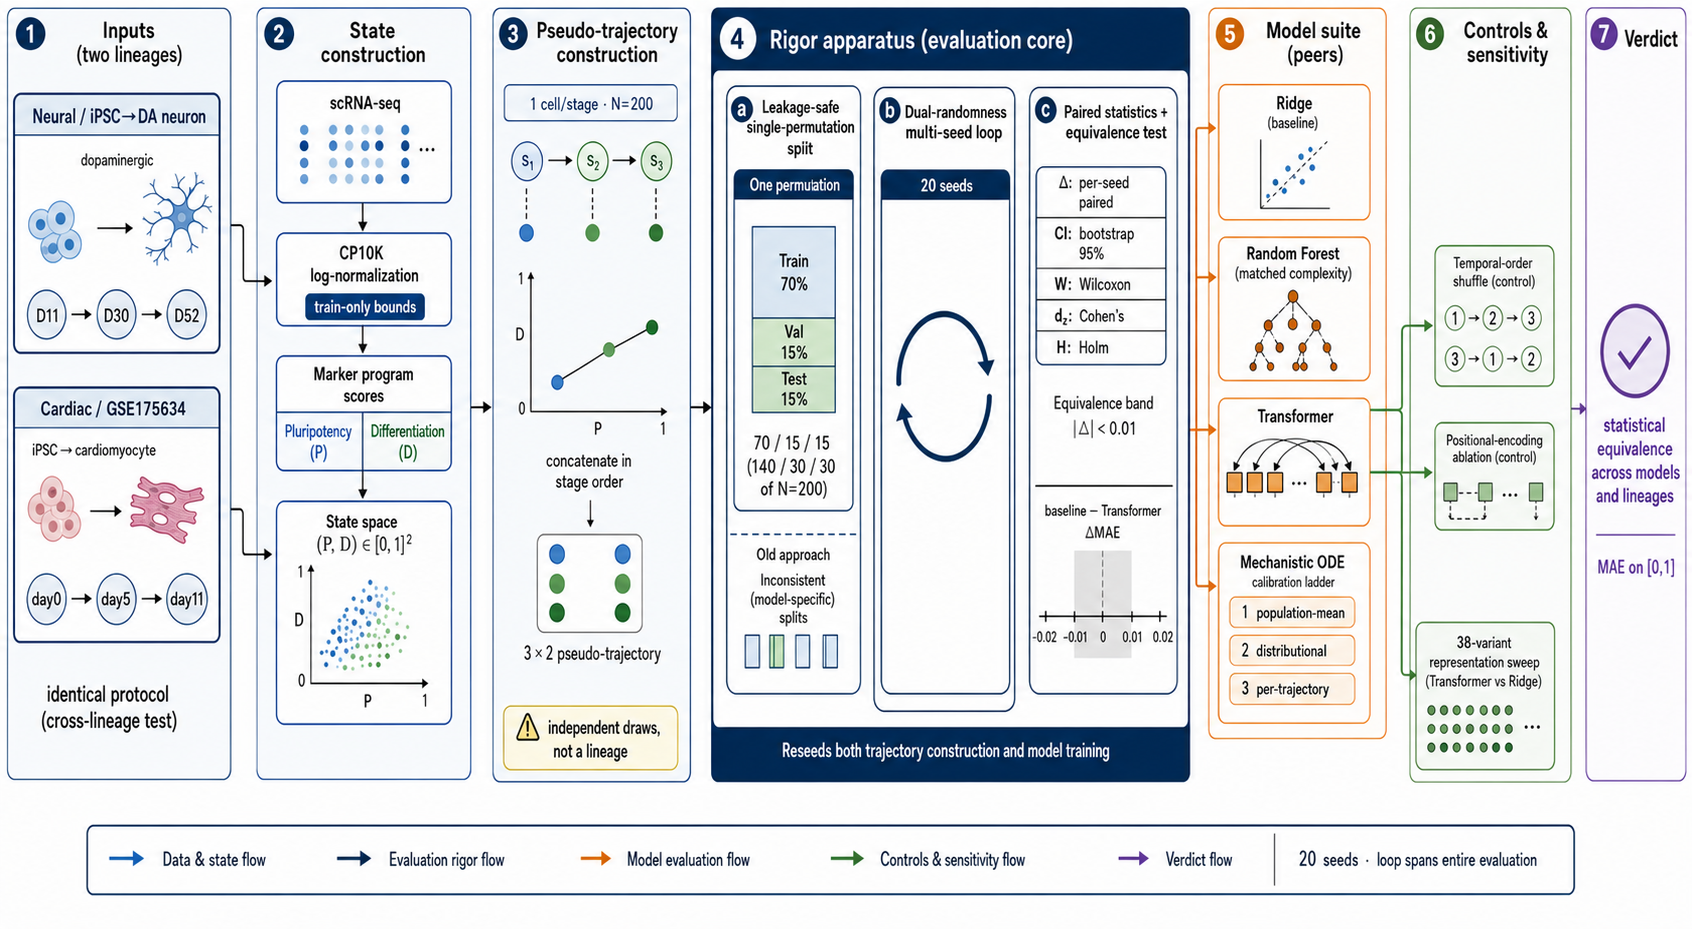
\includegraphics[width=\linewidth,height=0.78\textheight,keepaspectratio]{figures/method_design.png}
\end{column}
\begin{column}{0.41\textwidth}
\small
\begin{itemize}
\setlength{\itemsep}{0.6em}
\item{} Shared 70/15/15 split across every model
\item{} Training-only normalization and identical trajectories
\item{} Twenty seeds, paired statistics, bootstrap confidence intervals
\end{itemize}
\end{column}
\end{columns}
\end{frame}

\begin{frame}{Models and reference predictors}
\begin{itemize}
\setlength{\itemsep}{0.6em}
\item{} Ridge, random forest, Transformer, and mechanistic ODE
\item{} Constant mean matches the squared-error training objective
\item{} Constant median matches the absolute-error evaluation metric
\end{itemize}
\end{frame}

\begin{frame}{Controls test the benchmark itself}
\begin{itemize}
\setlength{\itemsep}{0.6em}
\item{} Stage-order shuffle and positional-encoding ablation
\item{} Thirty-eight marker-state representation variants
\item{} Simulated and optimal-transport positive controls
\end{itemize}
\end{frame}

\section{Key results}
\begin{frame}[plain]
\hxsectionslide{04}{Key results}
\end{frame}

\begin{frame}{Trained models are equivalent}
\begin{columns}[c]
\begin{column}{0.56\textwidth}
\centering
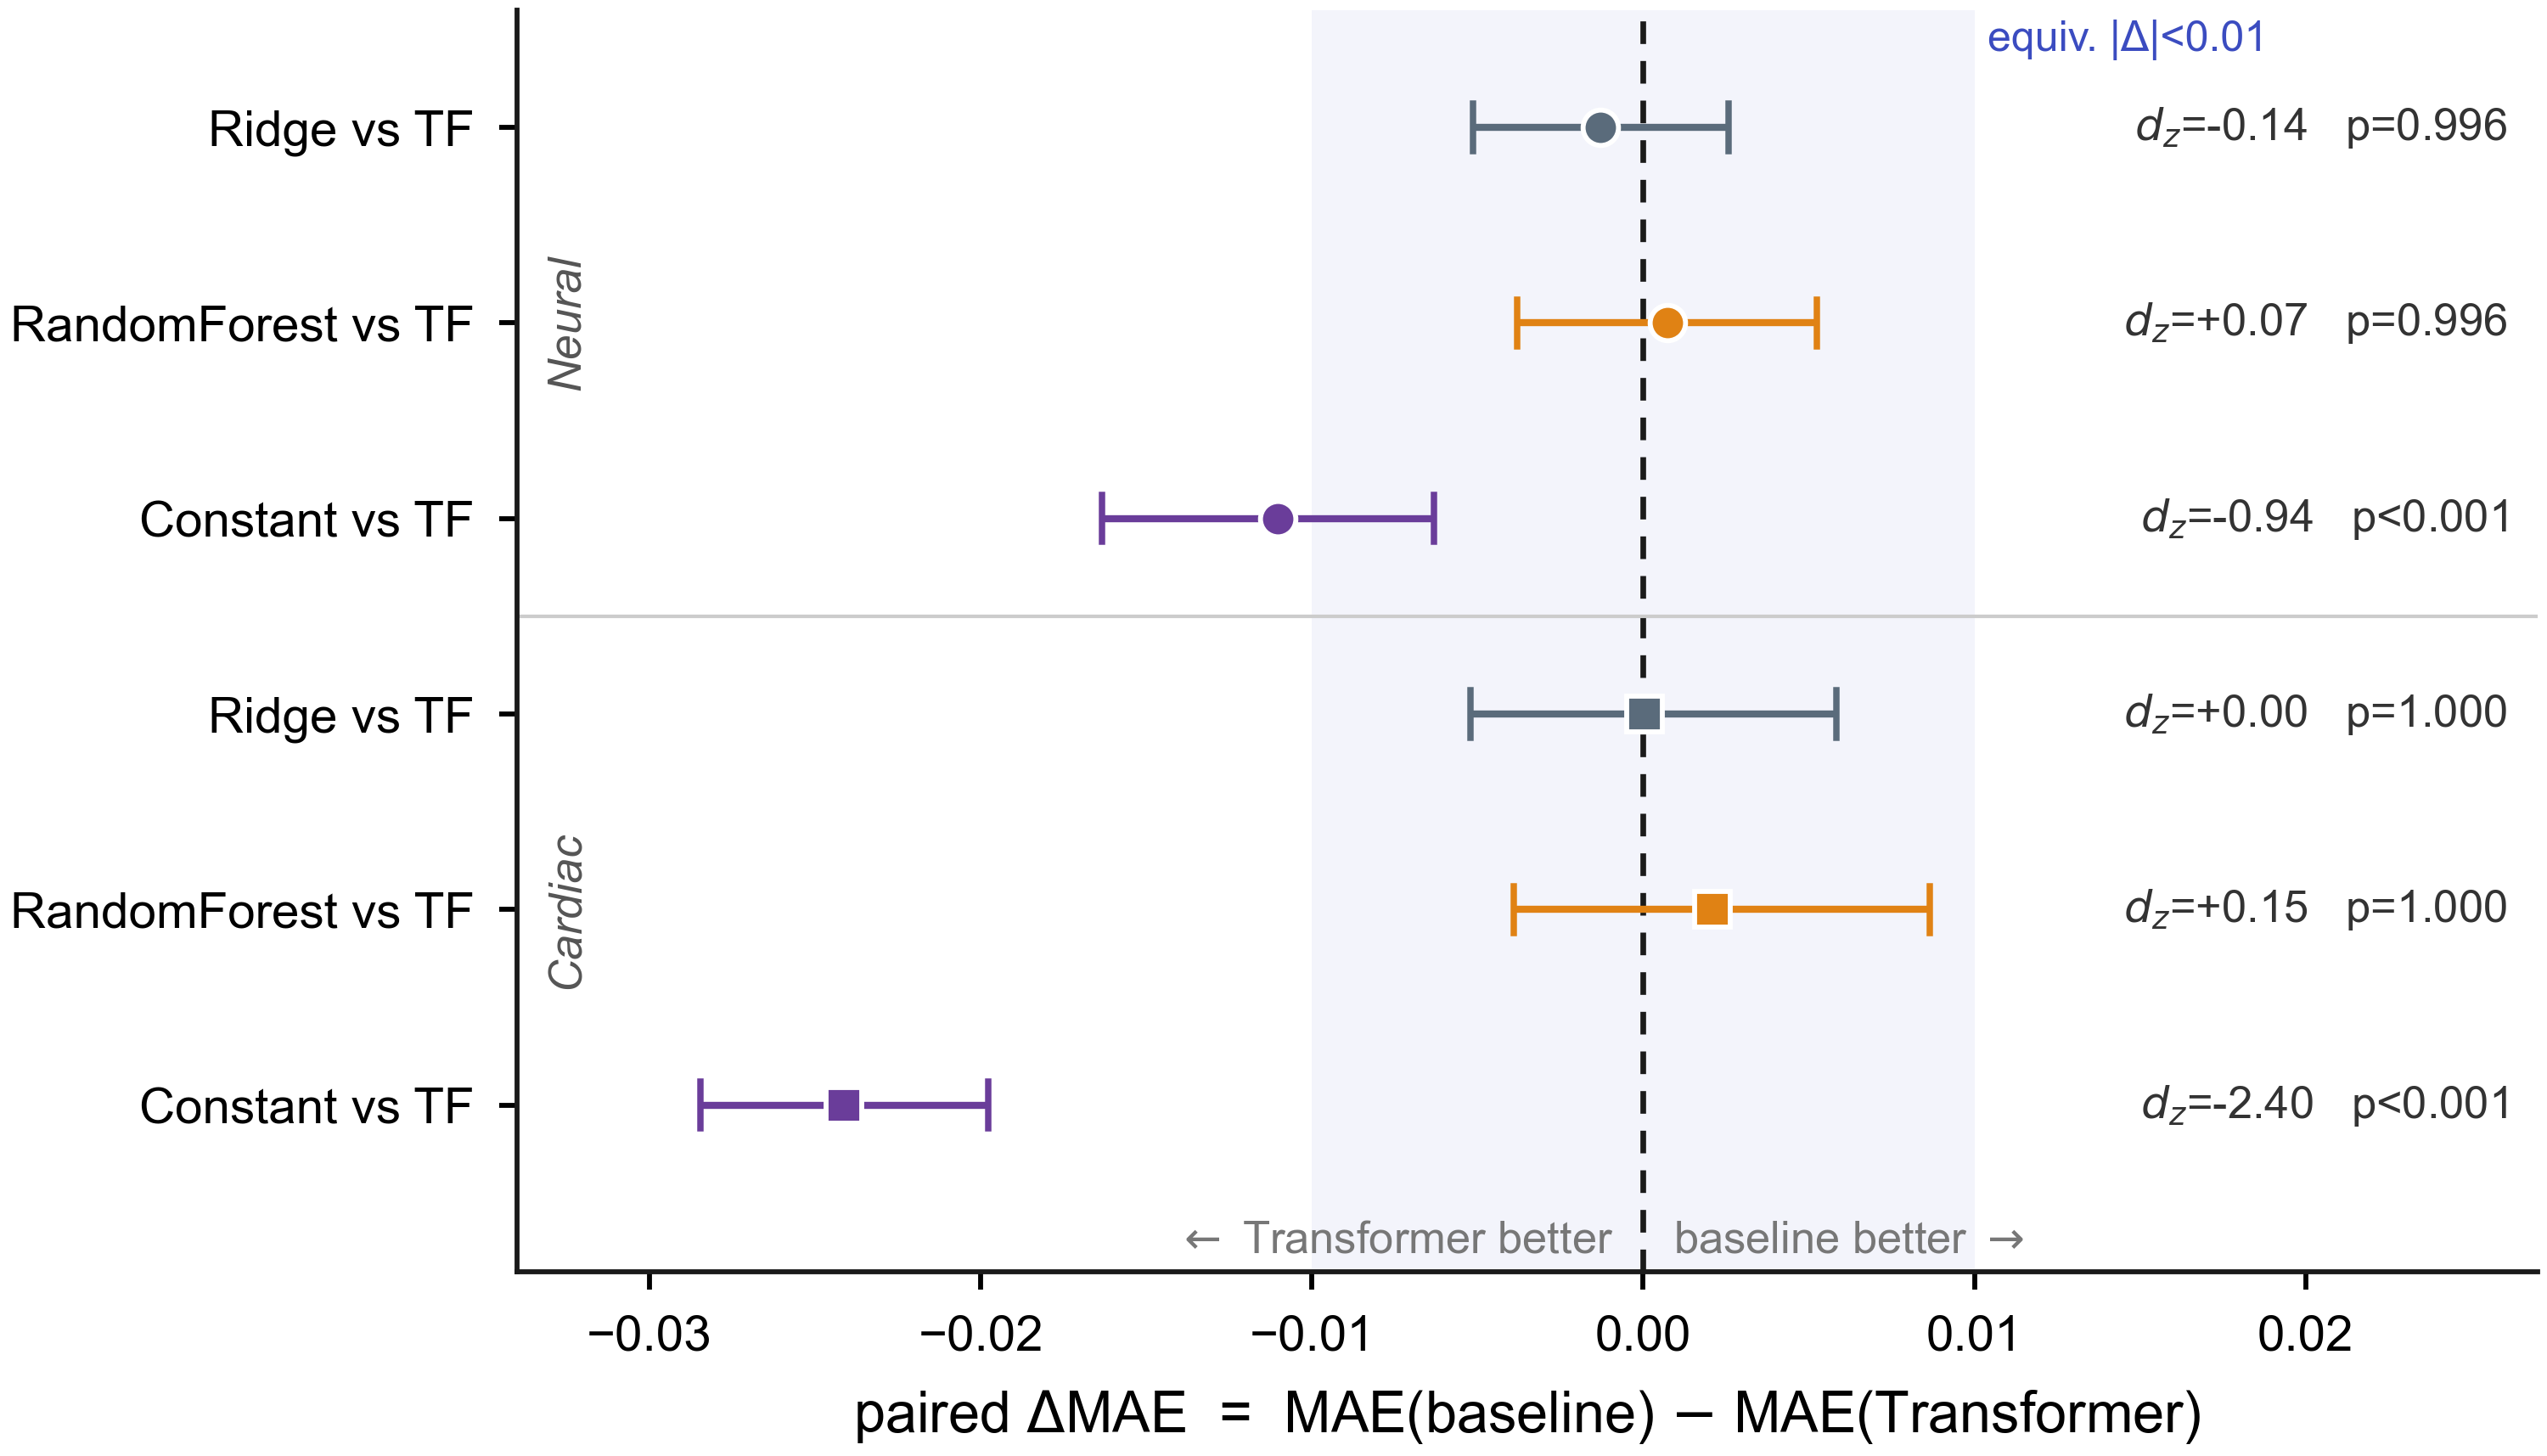
\includegraphics[width=\linewidth,height=0.78\textheight,keepaspectratio]{figures/fig2_forest.png}
\end{column}
\begin{column}{0.41\textwidth}
\small
\begin{itemize}
\setlength{\itemsep}{0.6em}
\item{} Neural MAE: Ridge 0.1774, forest 0.1794, Transformer 0.1787
\item{} Cardiac MAE: Ridge 0.1100, forest 0.1121, Transformer 0.1100
\item{} No trained model significantly outperformed another
\end{itemize}
\end{column}
\end{columns}
\end{frame}

\begin{frame}{The constant predictor wins}
\begin{columns}[c]
\begin{column}{0.56\textwidth}
\centering
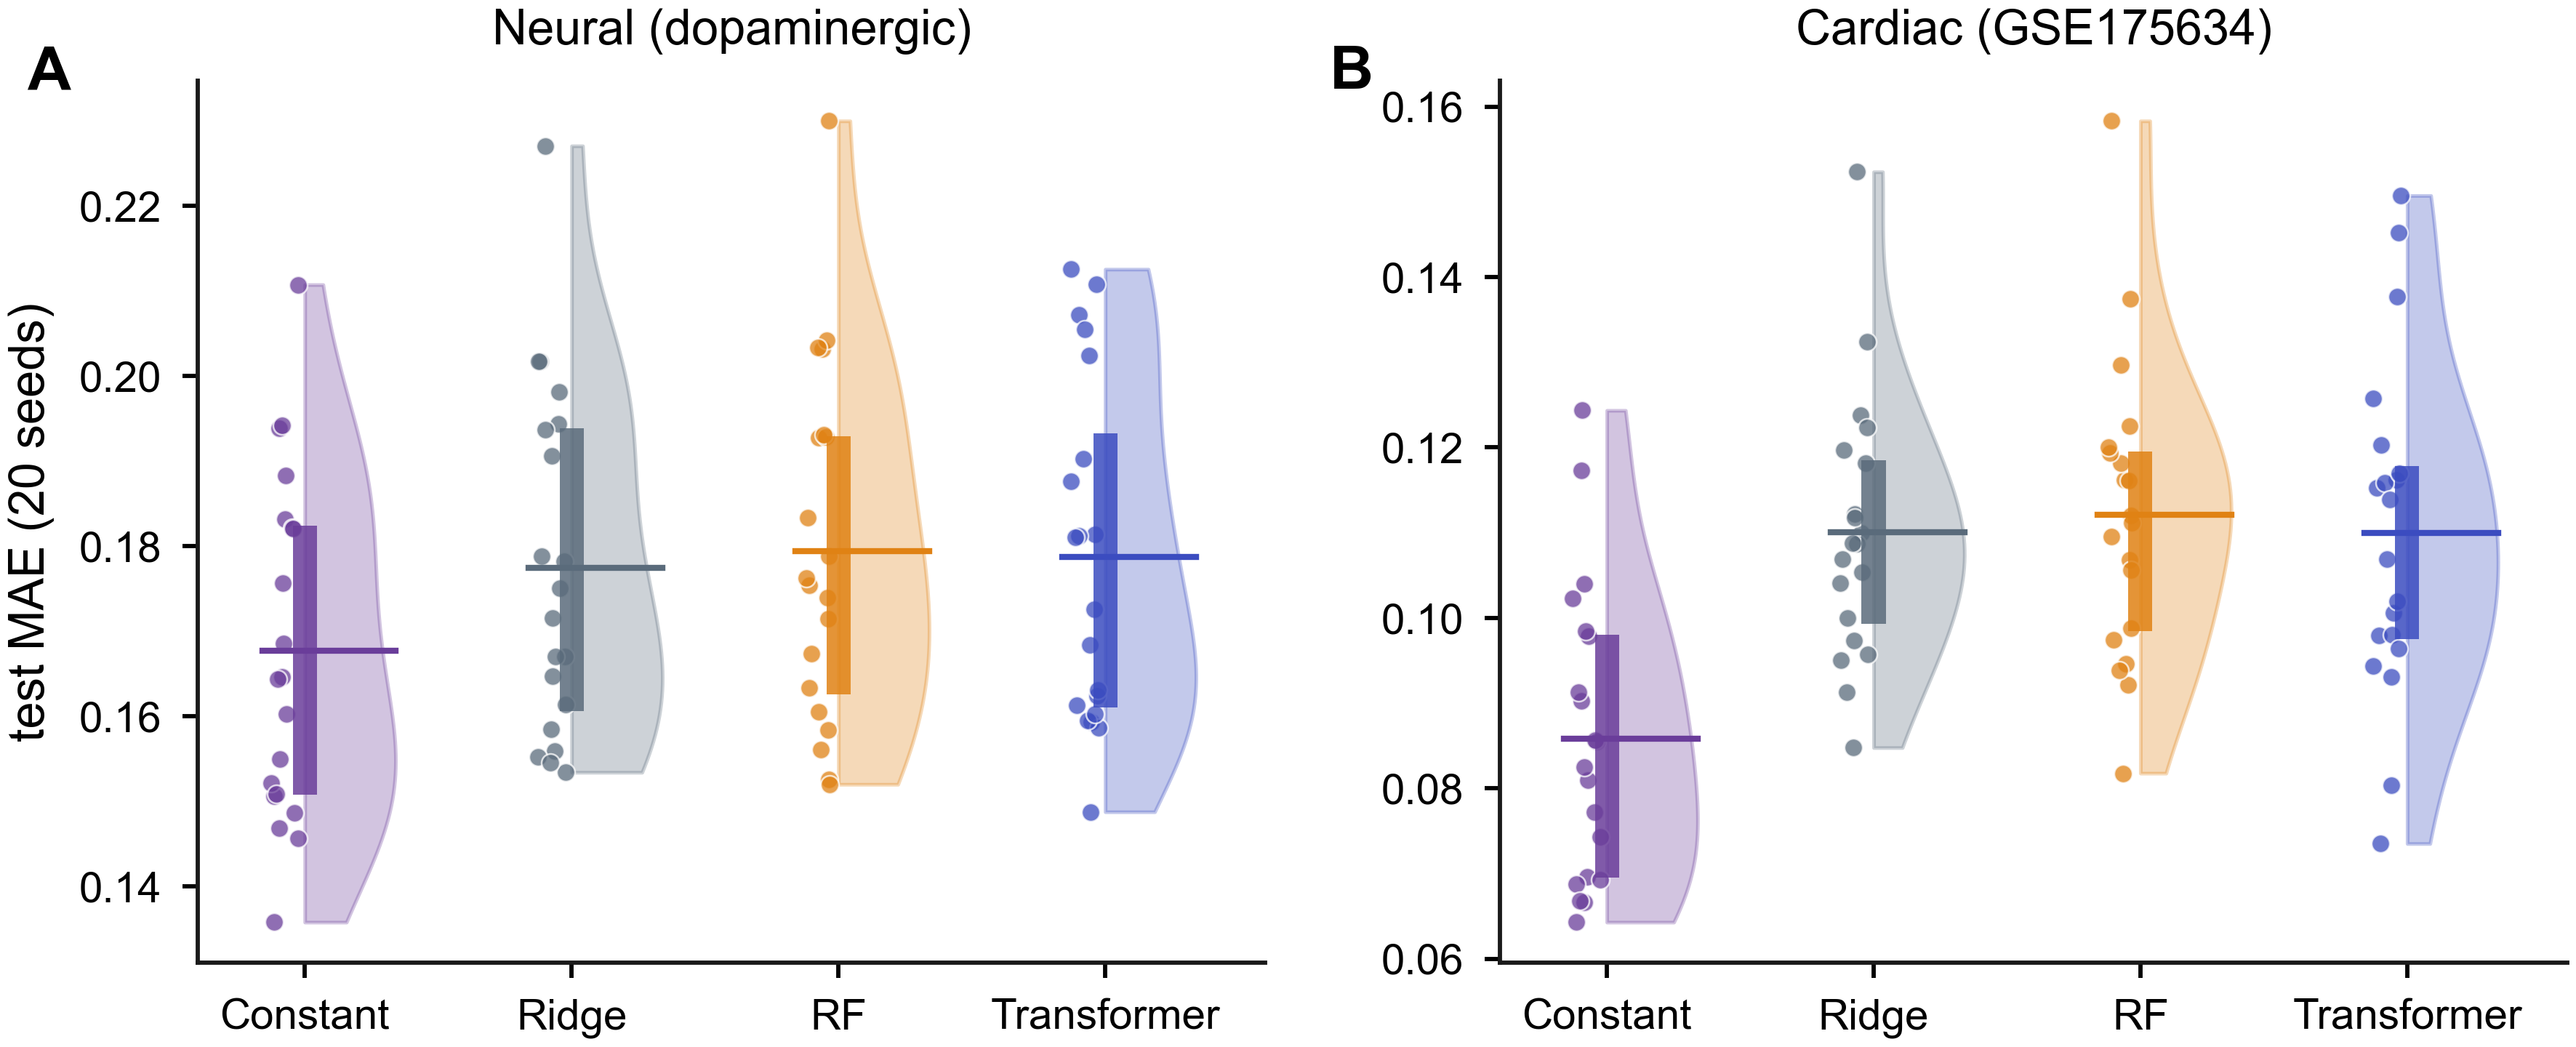
\includegraphics[width=\linewidth,height=0.78\textheight,keepaspectratio]{figures/fig3_raincloud.png}
\end{column}
\begin{column}{0.41\textwidth}
\small
\begin{itemize}
\setlength{\itemsep}{0.6em}
\item{} Training median beats every trained model
\item{} Neural improvement: 6--7\% lower error
\item{} Cardiac improvement: 28--31\% lower error
\end{itemize}
\end{column}
\end{columns}
\end{frame}

\begin{frame}{Leakage reverses the conclusion}
\begin{columns}[c]
\begin{column}{0.56\textwidth}
\centering
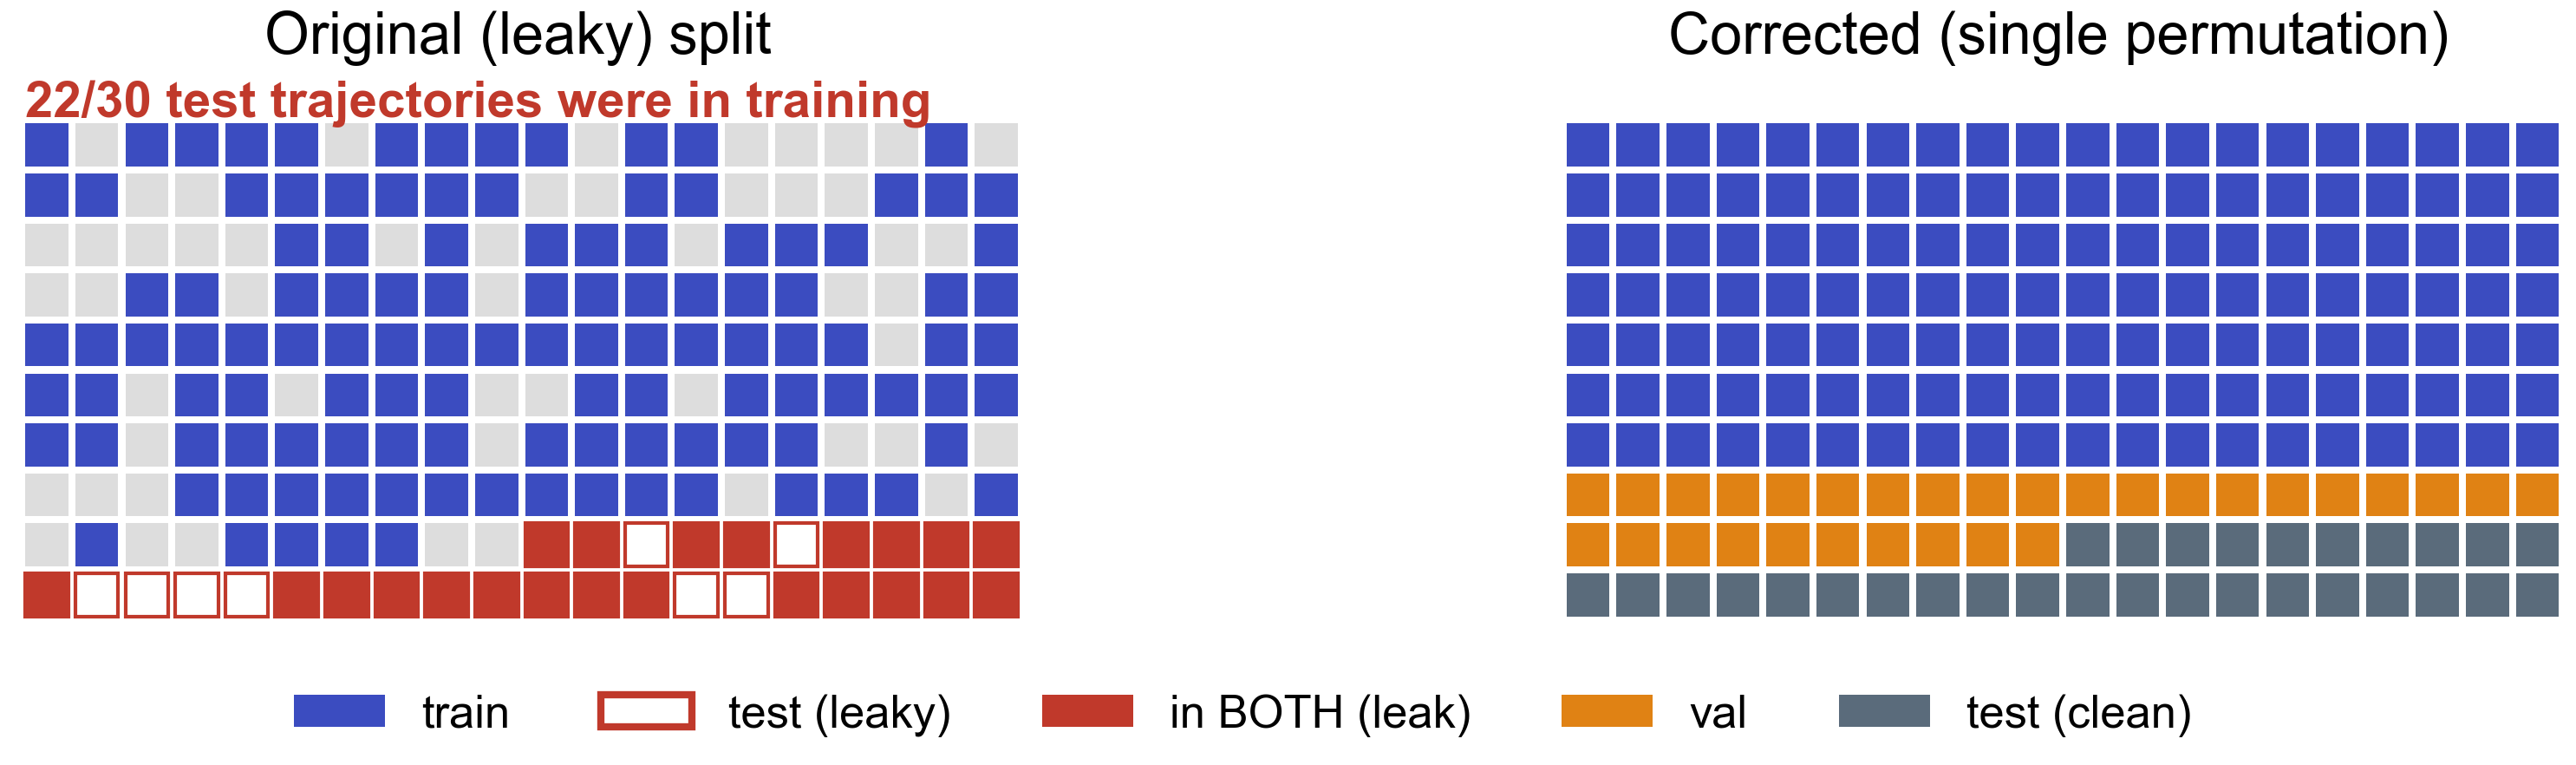
\includegraphics[width=\linewidth,height=0.78\textheight,keepaspectratio]{figures/fig1_leakage_panel.png}
\end{column}
\begin{column}{0.41\textwidth}
\small
\begin{itemize}
\setlength{\itemsep}{0.6em}
\item{} Leaky evaluation reported a 19.4\% Transformer advantage
\item{} Twenty-two of thirty Transformer test trajectories leaked into training
\item{} Consistent rescoring produced a 2.0\% Transformer deficit
\end{itemize}
\end{column}
\end{columns}
\end{frame}

\begin{frame}{Temporal controls are insensitive}
\begin{columns}[c]
\begin{column}{0.56\textwidth}
\centering
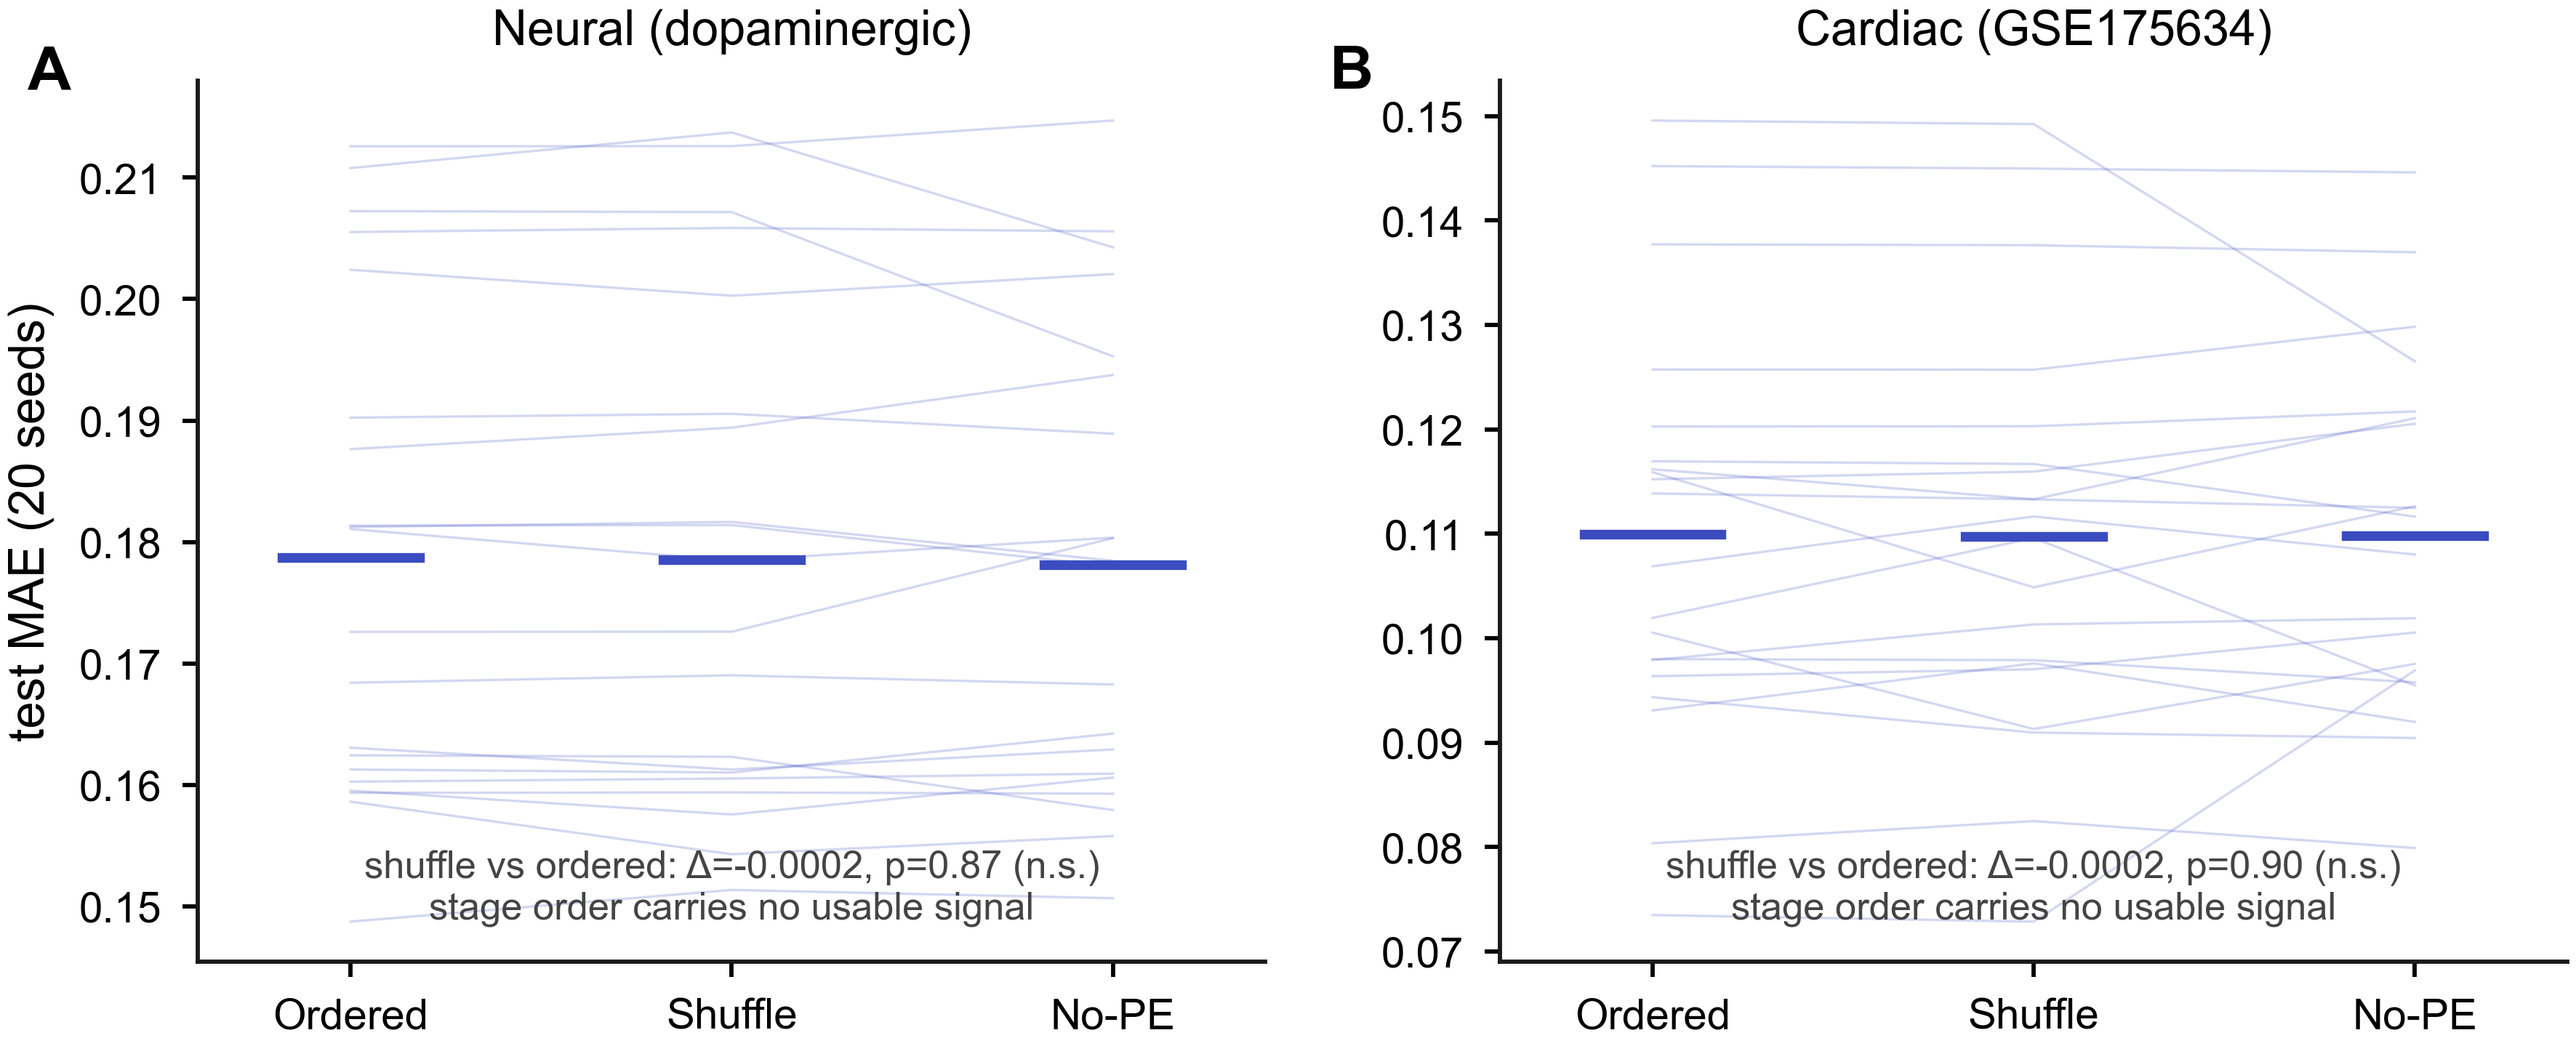
\includegraphics[width=\linewidth,height=0.78\textheight,keepaspectratio]{figures/fig4_temporal.png}
\end{column}
\begin{column}{0.41\textwidth}
\small
\begin{itemize}
\setlength{\itemsep}{0.6em}
\item{} Stage-order shuffle changed neural MAE by $-$0.0002
\item{} Shuffle effects were negligible relative to seed variability
\item{} Value differences can reveal stage identity without temporal order
\end{itemize}
\end{column}
\end{columns}
\end{frame}

\begin{frame}{Flexible ODE fitting worsens prediction}
\begin{columns}[c]
\begin{column}{0.56\textwidth}
\centering
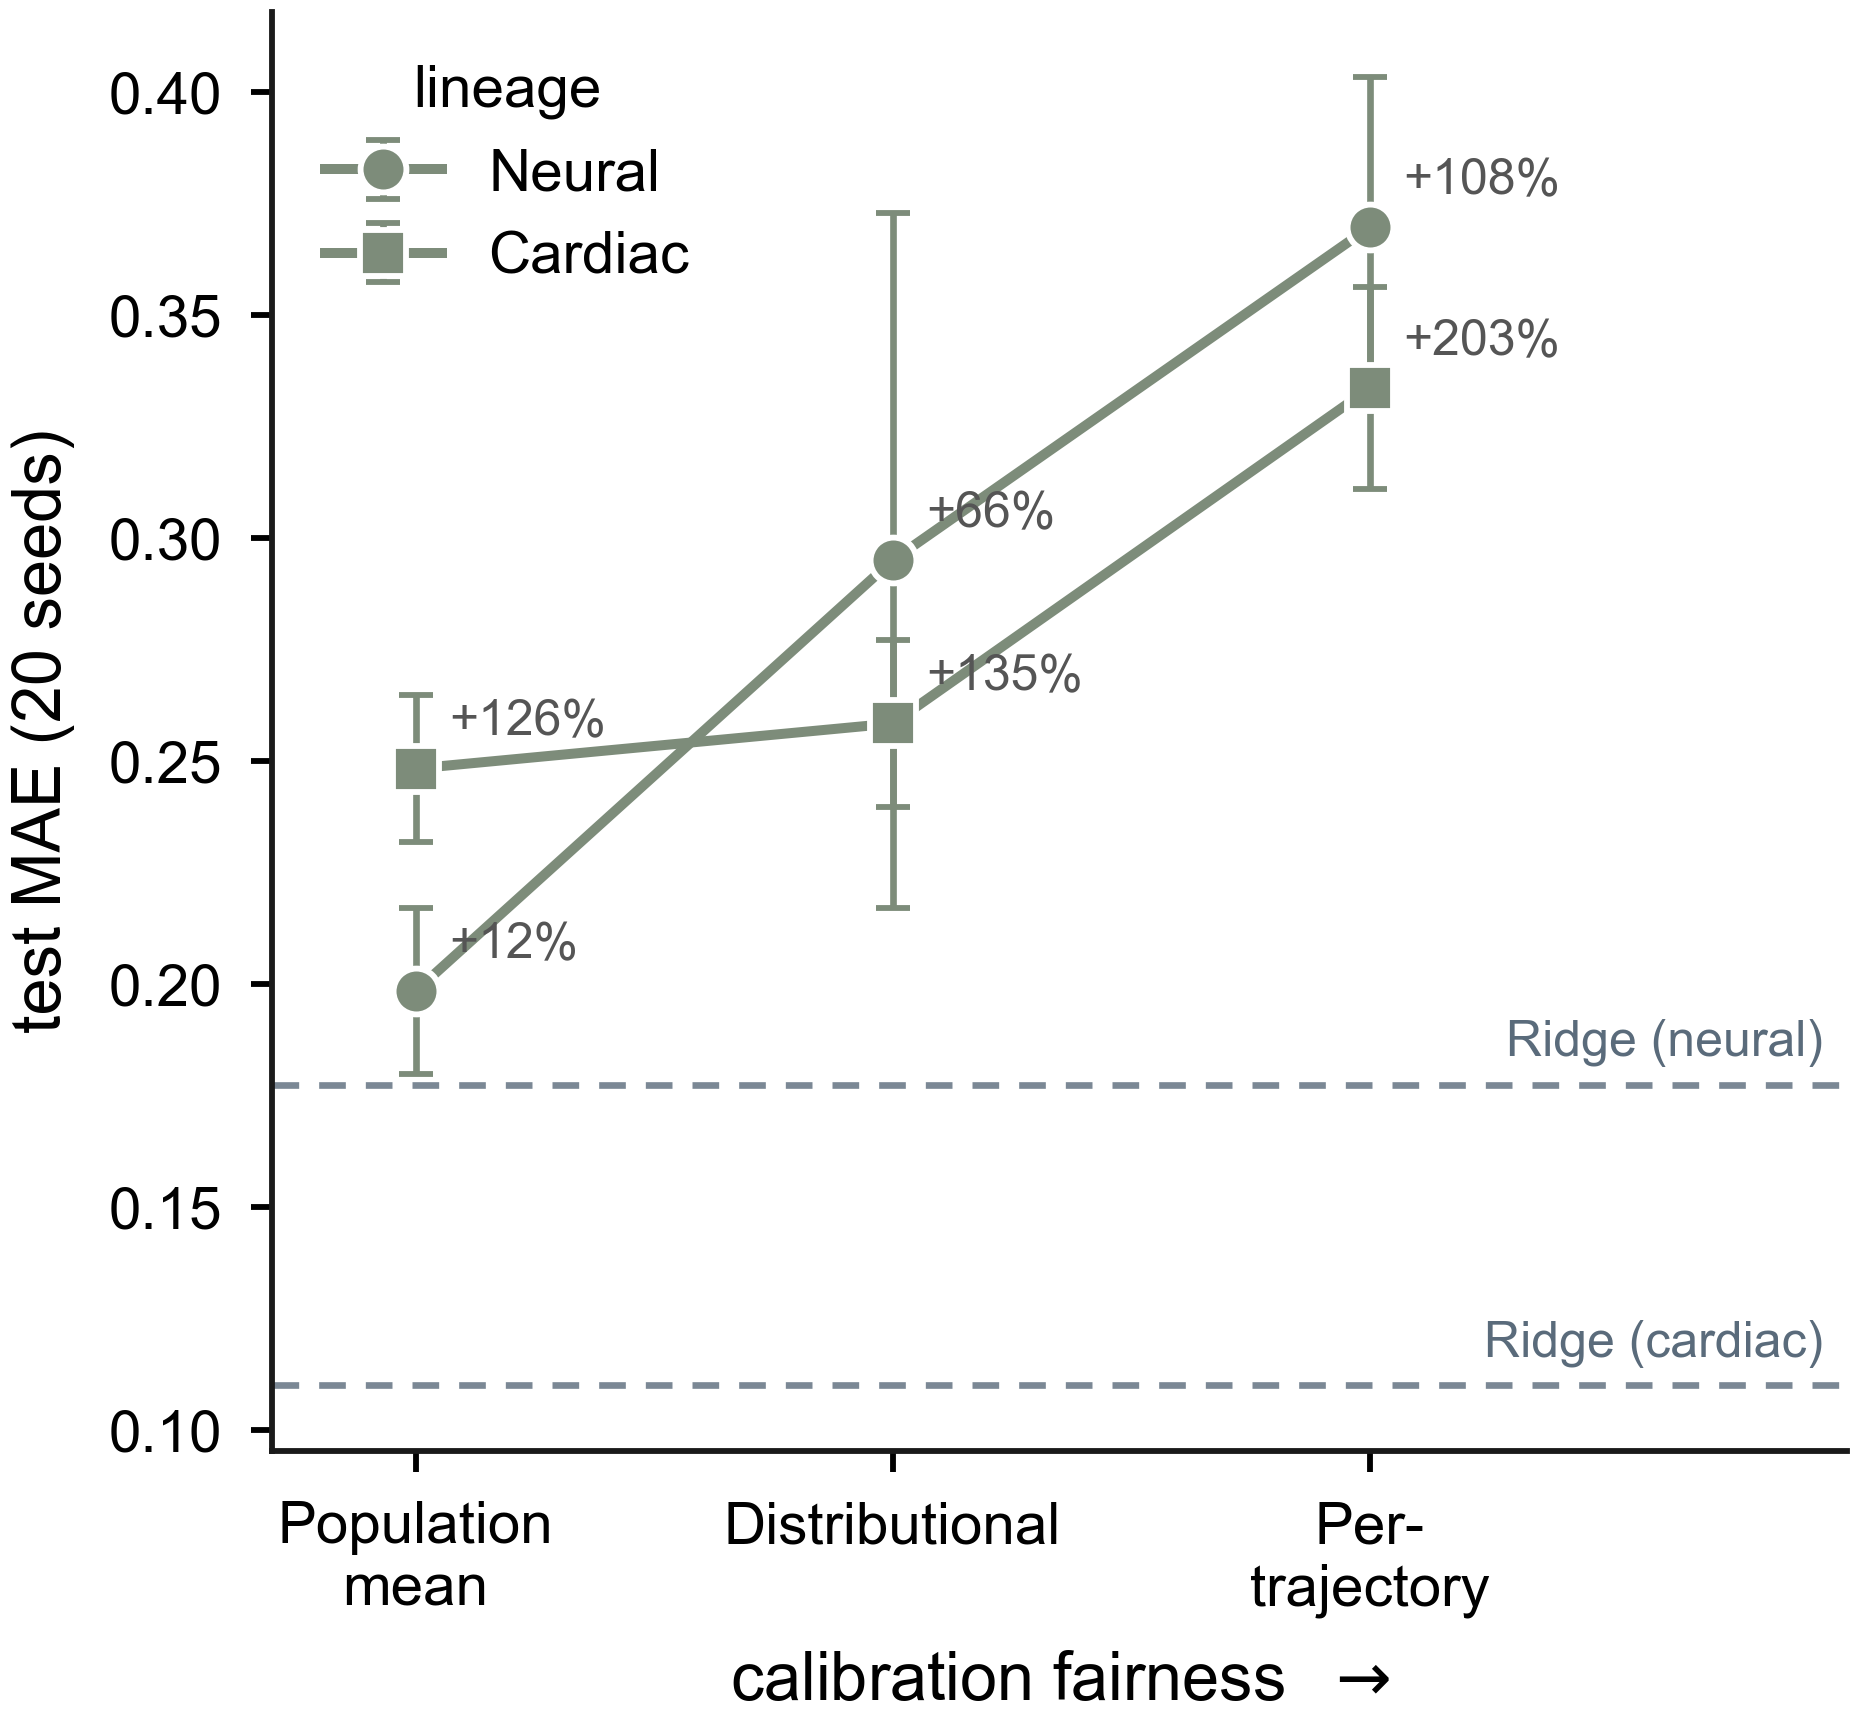
\includegraphics[width=\linewidth,height=0.78\textheight,keepaspectratio]{figures/fig5_ode.png}
\end{column}
\begin{column}{0.41\textwidth}
\small
\begin{itemize}
\setlength{\itemsep}{0.6em}
\item{} Neural ODE MAE rose from 0.198 to 0.370
\item{} Cardiac ODE MAE rose from 0.248 to 0.334
\item{} Fitting trajectory-level noise adds variance under the null
\end{itemize}
\end{column}
\end{columns}
\end{frame}

\begin{frame}{Positive controls recover dependence}
\begin{columns}[c]
\begin{column}{0.56\textwidth}
\centering
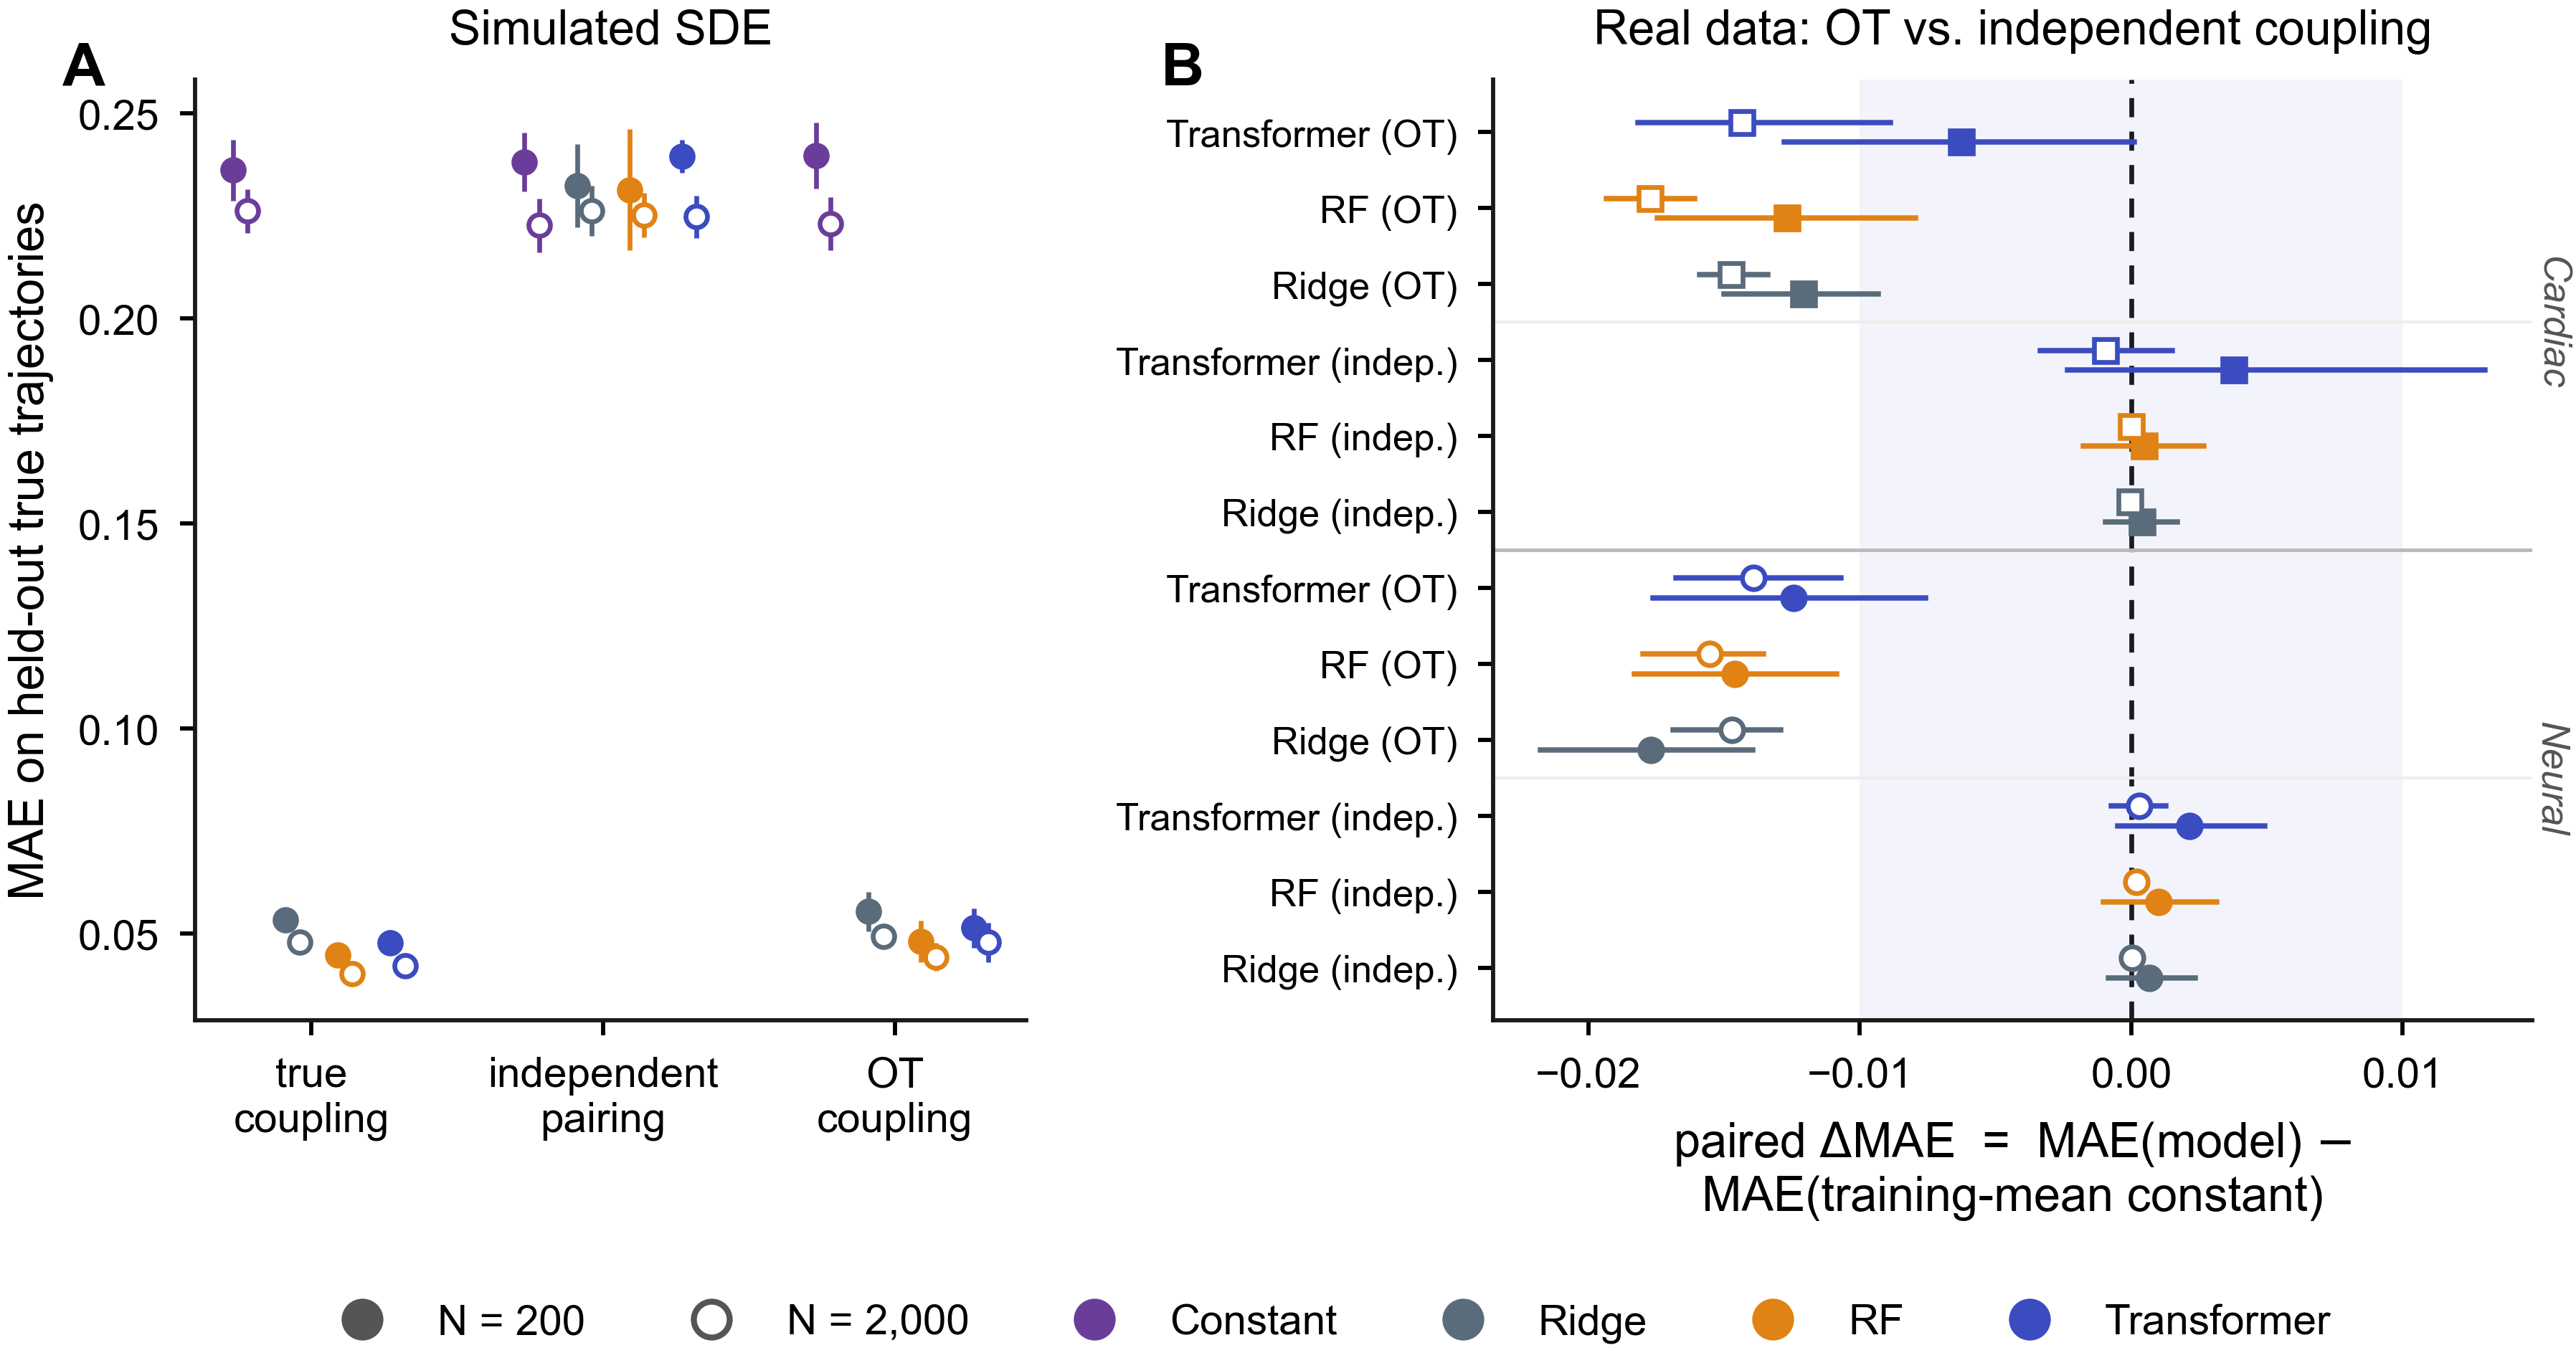
\includegraphics[width=\linewidth,height=0.78\textheight,keepaspectratio]{figures/fig7_positive.png}
\end{column}
\begin{column}{0.41\textwidth}
\small
\begin{itemize}
\setlength{\itemsep}{0.6em}
\item{} Independent pairing did not beat the constant
\item{} True and OT-coupled simulation reduced error substantially
\item{} The Transformer remained no better than the random forest
\end{itemize}
\end{column}
\end{columns}
\end{frame}

\begin{frame}{OT coupling changes real-data outcomes}
\begin{columns}[c]
\begin{column}{0.56\textwidth}
\centering
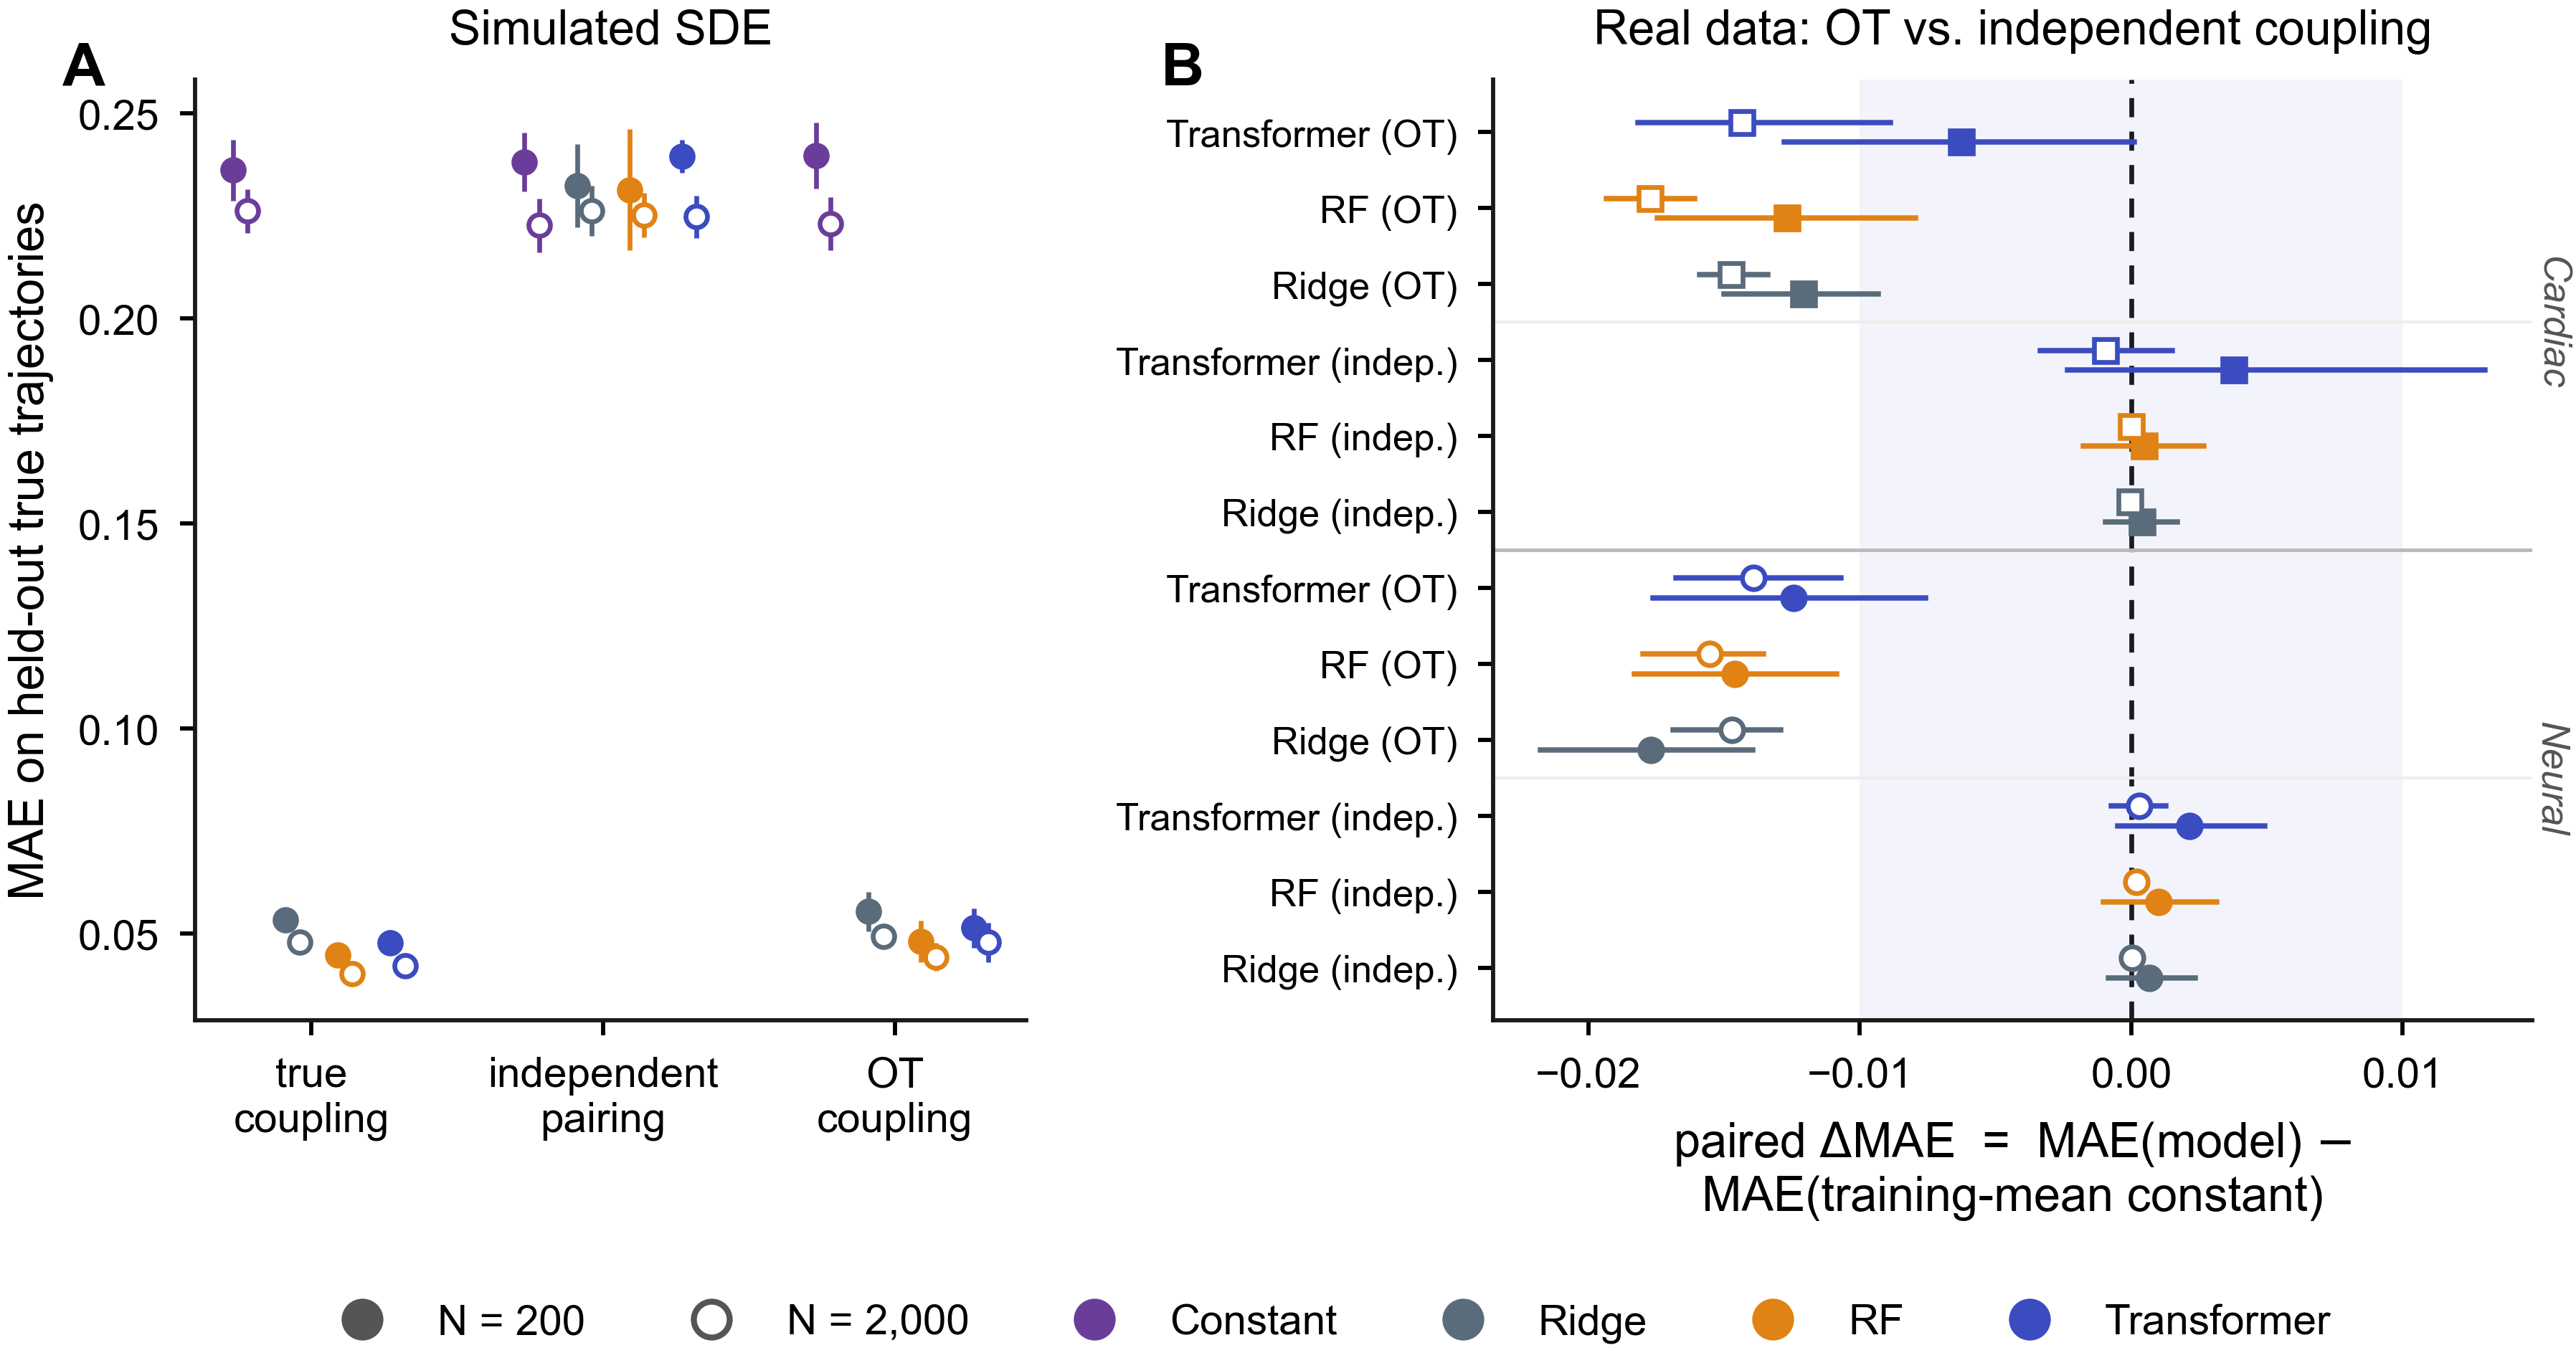
\includegraphics[width=\linewidth,height=0.78\textheight,keepaspectratio]{figures/fig7_positive.png}
\end{column}
\begin{column}{0.41\textwidth}
\small
\begin{itemize}
\setlength{\itemsep}{0.6em}
\item{} OT coupling let models beat the input-free baseline
\item{} The effect appeared on both real lineages
\item{} This demonstrates induced dependence, not biological validity
\end{itemize}
\end{column}
\end{columns}
\end{frame}

\section{Takeaways}
\begin{frame}[plain]
\hxsectionslide{05}{Takeaways}
\end{frame}

\begin{frame}{Coupling sets detectable signal}
\begin{itemize}
\setlength{\itemsep}{0.6em}
\item{} Independent pairing makes forecasting information unavailable
\item{} OT coupling introduces recoverable dependence
\item{} Model capacity cannot recover signal the benchmark removes
\end{itemize}
\end{frame}

\begin{frame}{Design better benchmarks}
\begin{itemize}
\setlength{\itemsep}{0.6em}
\item{} State explicitly how cells are coupled
\item{} Report a metric-matched input-independent baseline
\item{} Use shared splits, multiple seeds, and equivalence tests
\item{} Validate controls where dependence is known
\end{itemize}
\end{frame}

\begin{frame}{The main conclusion}
\begin{itemize}
\setlength{\itemsep}{0.6em}
\item{} Benchmark construction determines what forecasting can detect
\item{} The Transformer showed no advantage over simpler models
\item{} A benchmark must demonstrate both null recovery and signal detection
\end{itemize}
\end{frame}

\begin{frame}[plain]
\hxclosingslide{Thank you}{Questions?}
\end{frame}

\end{document}
